\chapter{Matching Of Impedances}
\verb|From| previous chapters, we have dealt with other applications of transmission lines. In this chapter we are going to learn about the  most important application of \textbf{Transmission Lines}, which is \textquotedblleft Impedance Matching\textquotedblright.
\begin{figure}[h]
\centering
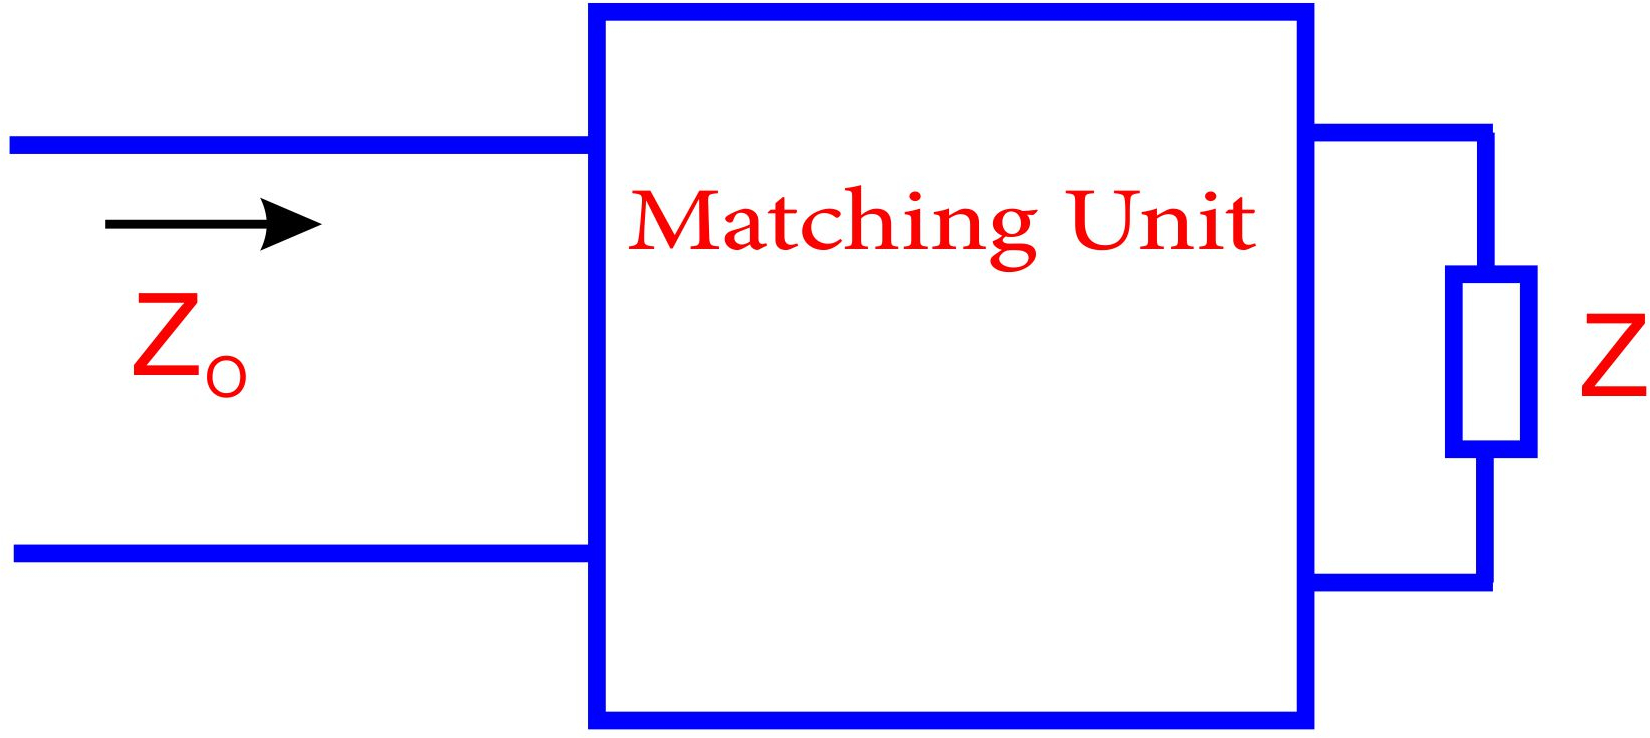
\includegraphics[width=1\linewidth]{./graphics/fig7}
\caption{Matching Transformer unit}
\end{figure} 

As we know from previous chapters, when impedance is equal to characteristic impedance $(Z_o)$, there is no reflection on the line, hence there is maximum power transfer. But as we have seen, this \textit{matching condition} is not always feasible. We then need a module or device which will transform this impedance to the characteristic impedance. This module  is known as a \textbf{matching unit or matching transformer}. 

Let's start with the first example which has a matching unit (transformer)  which can convert the output (Z) impedance to the characteristic impedance $Z_o$, which is shown in figure 12.1. At the input (left most side), we should see a characteristic impedance $ Z_o$ and the module should be completely lossless (ideal) to allow maximum power transfer to load($Z$).

Let's discuss various method by which different impedances can be matched to the characteristic impedance.
\begin{figure}[h]
\centering
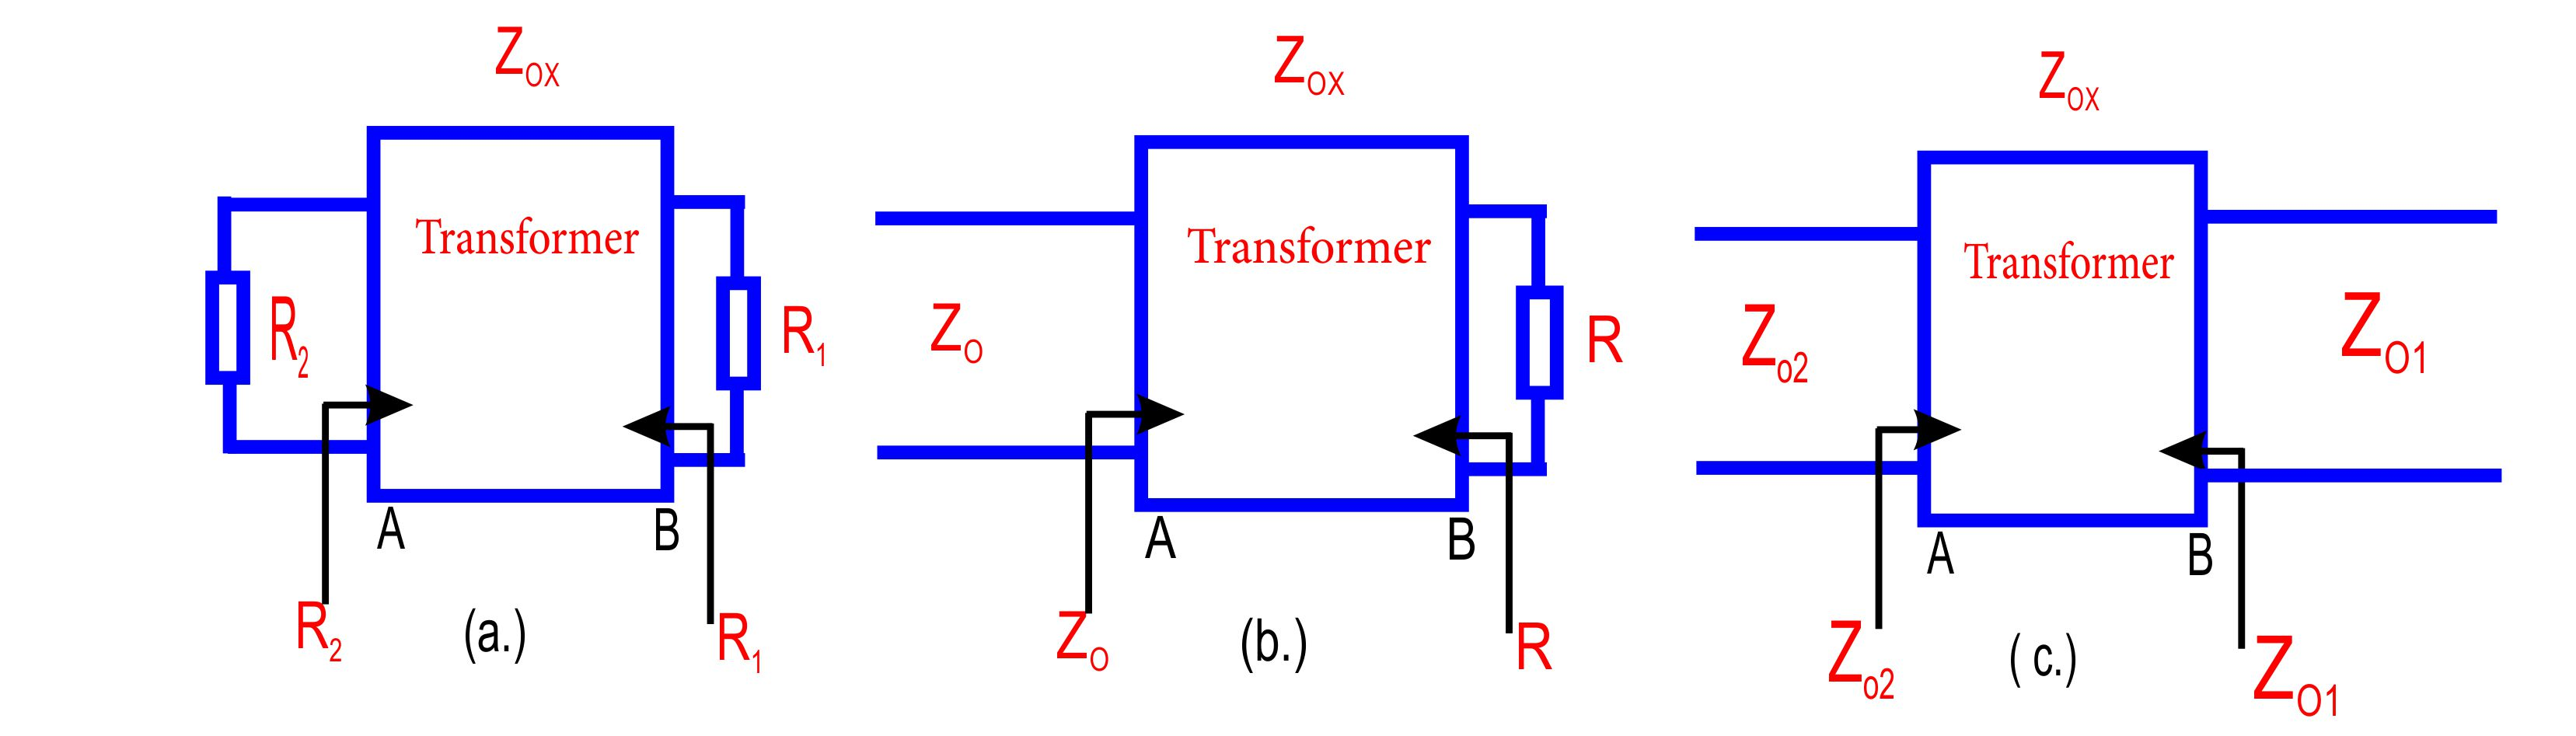
\includegraphics[width=1\linewidth]{./graphics/fig8}
\caption{Application of transformer}
\end{figure}
\verb| 	In| figure 12.2a we have two different resistance $R_1$ and $R_2$ which are to be matched, i.e $R_1\neq R_2$. If they are connected directly there will be a mismatch and no maximum power transfer from $R_1$ to $R_2$. We then introduce some  device in between that will make $R_1$ appear like $R_2$ when seen  from left side and $R_2$ to appear like  $R_1$, when seen from the right side, so from both side it will appear that they are matched to the load and there is maximum power transfer.

In figure 12.2b, we are matching R to $Z_o$, so we place in a module which help us to match the impedances between R and $Z_o$. Hence at the left side we should see $ Z_o$

Also in figure 12.2c, which is the most important case. We have two(2) long transmission lines which are to be connected together. If the length of each transmission is very large, the input impedance of transmission line one(1) will appear as its characteristics impedance ($ Z_{o1}$) and transmission line two(2) will appear as its characteristics impedance $ Z_{o2}$. Making a straight connection between them,  $ Z_{o2}$ sees itself connected to $ Z_{o1}$ and vice-versa. This will cause an impedance mismatch and reflection towards both side at the junction of transmission line. So we bring a transforming device in between that will make  $Z_{o1}$ see $Z_{o2}$ as $Z_{o1}$ and vice-versa. From both sides, it seems as if the line is terminated in its characteristic impedance. Hence there will be no reflection on either side of the transmission line.

\section{Quarter Wavelength Transformer Technique}
On the smith chart, if we have an impedance which is resistive, how much can we move on the transmission line so that the impedance always appear like a resistance? Let us introduce some section of transmission line in between both impedances (input and output) which have a characteristic impedance $ Z_{ox}$ in figure 12.2a and 12.2b  and is different from the characteristic impedance  $ Z_o$ to which the resistive impedance R is to be matched.

Hence, we find out $ Z_{ox}$ and the length of this introduced transmission line for which R can be matched with $ Z_o$. Resistive impedance lie on the horizontal axis of the smith chart, $Z >  Z_o$ lies on the right and $Z <  Z_o$ lies on the left of smith chart.
So the question is: What should be the value of $Z_{ox}$ and length l, that will match the resistive impedance to the characteristic impedance( $Z_o$)? From the smith chart shown in figure 12.3, to see a resistance again, we move $ \lambda/4$  or $ \lambda/2$. % remember to put in a smith chart here%
\begin{figure}[h]
\centering
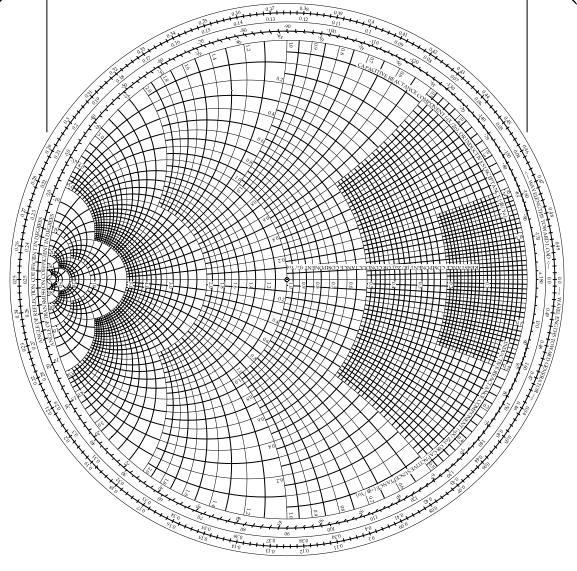
\includegraphics[width=1\linewidth]{./graphics/smich}
\caption{Smith chart}
\end{figure}
$\lambda/2$ movement brings us back to the same impedance. We won't use this value because it will transform the impedance to itself. $\lambda/4$ movement will have a resistive impedance which is different from the original resistive impedance(i.e inverts itself). $l = \lambda/4 $ will be most appropriate because at this length we will have a different resistive value.\\%remember to put in a figure here%
\begin{figure}[h]
\centering
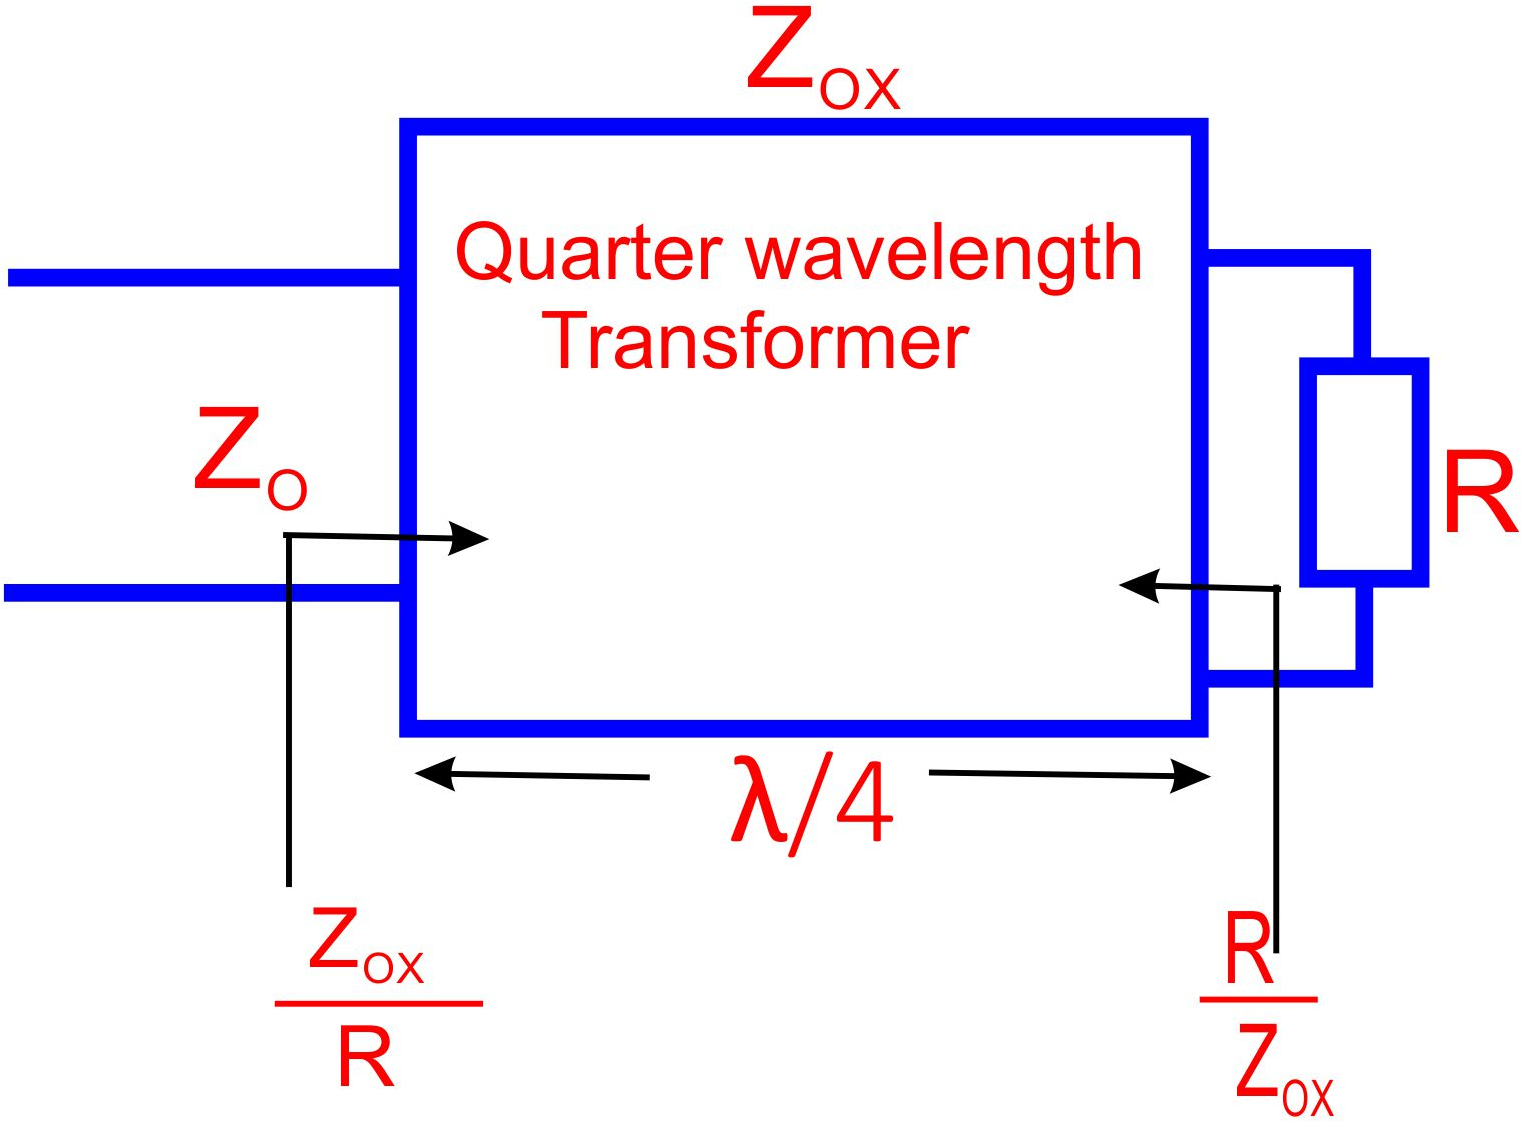
\includegraphics[width=1\linewidth]{./graphics/fig9}
\caption{The quarter wavelength transformer technique}
\end{figure}
From figure 12.4, at the transformer (output), the normalize impedance seen will be $R/Z_{ox}$. At the transformer(input), the normalize impedance seen will be $Z_{ox}/R$ (we know from property of transmission line, that every distance of $l = \lambda/4$, the impedance inverts itself). So the absolute characteristic impedance($ Z_o$) seen at the input will be equal to: 
\[
Z_o=(Z_{ox}/R)\times Z_{ox}\]  which gives 
\[ Z_o=(Z_{ox}^2/R)\]
therefore, \begin{equation}
Z_{ox}=\sqrt{RZ_o}
\end{equation}

What does this tell us? This equation tells us that if we have a mismatch condition, we can input a matching transformer ( an example is the BALUN)\footnote{A BALUN is a device which is use to connect balance load to an unbalance load, it is mostly use in television.  it has a length ($L=\lambda/4$), and a characteristic impedance $Z_{ox} $}.
Introducing this section of transmission line, we will have a matched condition where R will appear as $ Z_o$ when seen from the input and $ Z_o$ will appear as R when seen from output. Since line is lossless, there is a match on the transmission line from $ Z_o$ to R, therefore, we will see a maximum power transfer.
This technique of matching impedance is known as the\\ 
\underline{\textbf{Quarter Wavelength Transformer Technique}} which derives its name from the fact that we have to travel a length which is equal to a quarter, i.e 1/4 of the wavelength($\lambda$). This matching transformer is also used for matching lumped circuit.\\
\subsection{Complex load impedance}
\verb| 	A| question may be asked: if this technique(quarter wavelength transformer technique) is only used to match resistive impedance? The answer is absolutely \textbf{No!}  We can use this method to solve complex impedances but it requires us to do some thinking because on the first look, it appears impossible. This is because on the smith chart shown in figure 12.3, to derive $Z_{ox}$, we use only the horizontal axis of the chart. Now, how can we use both the real and imaginary parts of the chart?

As we saw earlier, we need to do some proper thinking to solve complex load(Z). We solve it  by first transforming the complex  normalized impedances to a real impedance by moving along the length of a transmission line. That means if you introduce some length of transmission line with characteristic impedance ($ Z_o$), then the impedance seen at the other end is real if the length is such that you get a voltage (maximum or minimum) for that length.
\begin{figure}[h]
\centering
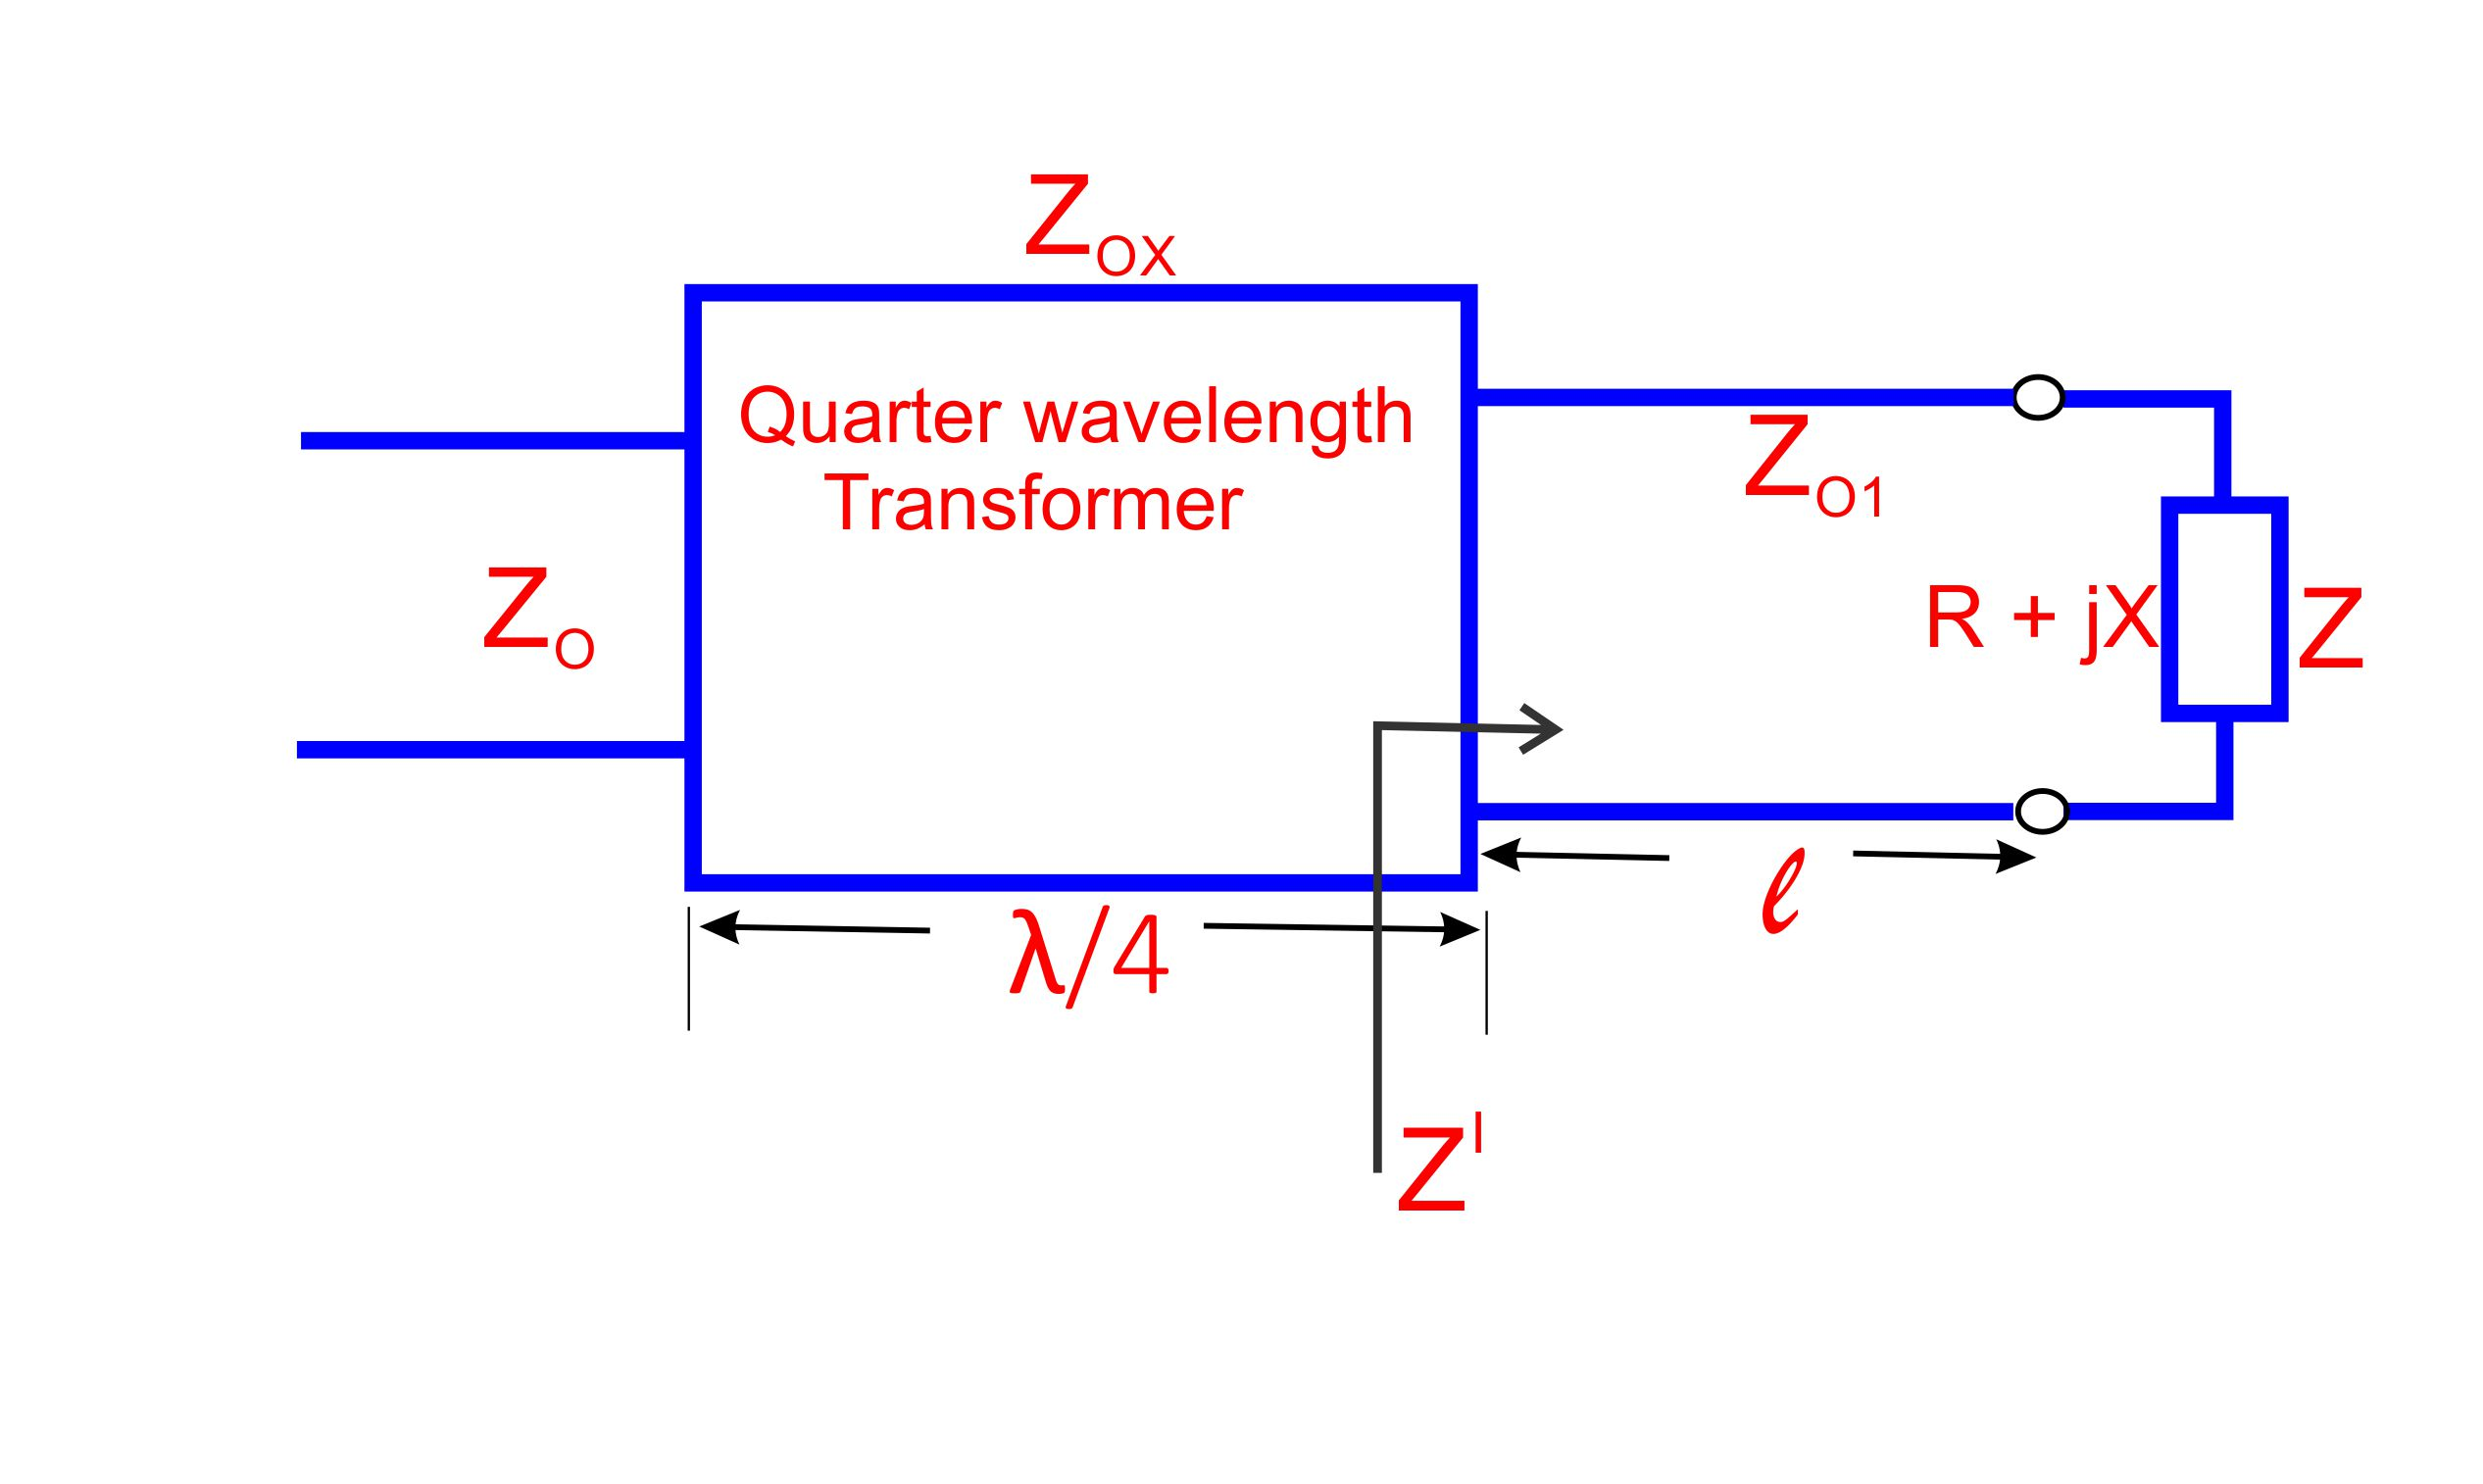
\includegraphics[width=1\linewidth]{./graphics/fig10}
\caption{The quarter wavelength transformer technique for complex load Z}
\end{figure}

From figure 12.5, we have to move $ Z$ which is complex by a distance l on the transmission line to make its transformed impedance real at point B.
\begin{figure}[h]
\centering
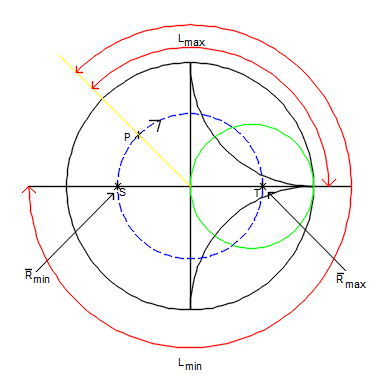
\includegraphics[scale=0.6]{./graphics/sinsmith}
\caption{ Simplified smith chart for complex load Quarter wavelength transformer }
\end{figure}

\verb|U|sing analytical method may be time consuming and tedious, so we use a smith chart to solve the problem.\\ 
\underline{\textbf{ Procedures:}}
\begin{enumerate}
\item Let $ Z = R + jX$ normalized become point $ P= \overline{R} +$ \footnote{The normalised impedance $ \overline{Z}$ is normalized with respect to characteristic impedance of the line $ Z_{o1}$, that is $ \overline{Z} = Z/ Z_{o1}$} $j\overline{X}$  on the smith chart shown in figure 12.6.
\item  From point P, draw a constant VSWR circle.
\item As we move on a constant VSWR circle (clockwise), we reach a point T which is a real impedance $\overline{R}_{max}$. As we move further, we reach a point S which is also a real impedance $\overline{R}_{min}$.
\item $ l_{max}$ represents the distance from point P to T, while $ l_{min}$ represents the distance from point P to S.
\item If we know the VSWR ($\rho$), the normalized impedance at point T and S would be known.
\item considering distance  $ l_{max}$, the absolute impedance ($ Z'$) seen at point T is \begin{equation}R_{max} = Z_{o1}\times\rho
\end{equation}
\item considering distance  $ l_{min}$, the absolute impedance ($ Z'$) seen at point S is\begin{equation} R_{min} = Z_{o1}/\rho\end{equation}
\item Therefore the absolute impedance ($Z'$) at point B in figure 12.5 can be found using either $ R_{max}$ or $ R_{min}$.
\end{enumerate}

Therefore the characteristics impedance of the quarter wavelength transformer $Z_{ox}$ would be: 
\begin{equation}
\boxed{Z_{ox}=\sqrt{Z_{o1}\rho Z_o}} 
\end{equation}
\\OR
\begin{equation}
\boxed{Z_{ox}=\sqrt{Z_{o1}Z_o/\rho}}
\end{equation}

Any solution is acceptable depending on whether we want the length $l$, to be small or large. If we are taking cost into consideration, we will choose for shorter length of the transmission line.\\

In conclusion, we can say that\textit{ Quarter Wavelength Transformer technique} can be used for matching complex impedance (Z) to real impedance($Z_o$). However, it has a big drawback in that you require a unique characteristic impedance $Z_{ox}$ for the transforming device for different load Z. This is not desirable and realizable in nature because in practice, we do not get a\textit{ Transmission Line} whose characteristic impedance can be varied easily. The characteristic impedance $Z_{ox}$  depends on the physical dimensions of the transmission line as will be seen in chapter 15. We have cables of transmission line with standard characteristic impedance. For example for co-axial cable, the characteristic impedances are 50$\Omega$ and 75$\Omega$. For parallel wire transmission line, the characteristic impedances are 300$\Omega$ and 600$\Omega$.\\
\verb|The| question then is, can we use the standard transmission line which are available with their standardize characteristic impedances?
\section{Stub Matching Technique}
\verb|T|he answer to section 12.1 question is \textbf{Yes!} The approach used in solving this problem is known as \textbf{Stub Matching Technique}. Let's define a Stub.\\

A stub is an auxiliary section of a transmission line which is either short circuited (S.C) or open circuited (O.C), appended or connected to the main transmission line either in series or parallel. There are four(4) types of stub matching technique, which are :\\
\begin{enumerate}
\item Series O.C stub matching technique
\item Series S.C stub matching technique
\item parallel O.C stub matching technique
\item Parallel S.C stub matching technique
\end{enumerate}
In this chapter, we are going to be concentrating on the \textbf{Parallel Short Circuit Stub Matching Technique.}\\

By using the stub at proper location on the main transmission line, it is possible to match a complex impedance(Z) to the characteristic impedance ($Z_o$).\\
\underline{Note}: We do not require a unique characteristic impedance ($Z_o$) for each impedance matching. The characteristic impedance of the main and auxiliary transmission line remains the same.\\

What we want to change now is the length $l$ from load (location of stub) and the length of the auxiliary transmission line attached to the main transmission line ($l_s$). There are three (3) techniques for appending an auxiliary line (stub) to the main line. They are :
\begin{enumerate}[(i)]
\item Single Stub matching technique - One appended auxiliary line.
\item Double Stub matching technique - Two appended auxiliary line.
\item Triple Stub matching technique - Three appended auxiliary line.  
\end{enumerate} 
\subsection{Single Stub Matching Technique }
\begin{figure}[h]
\centering
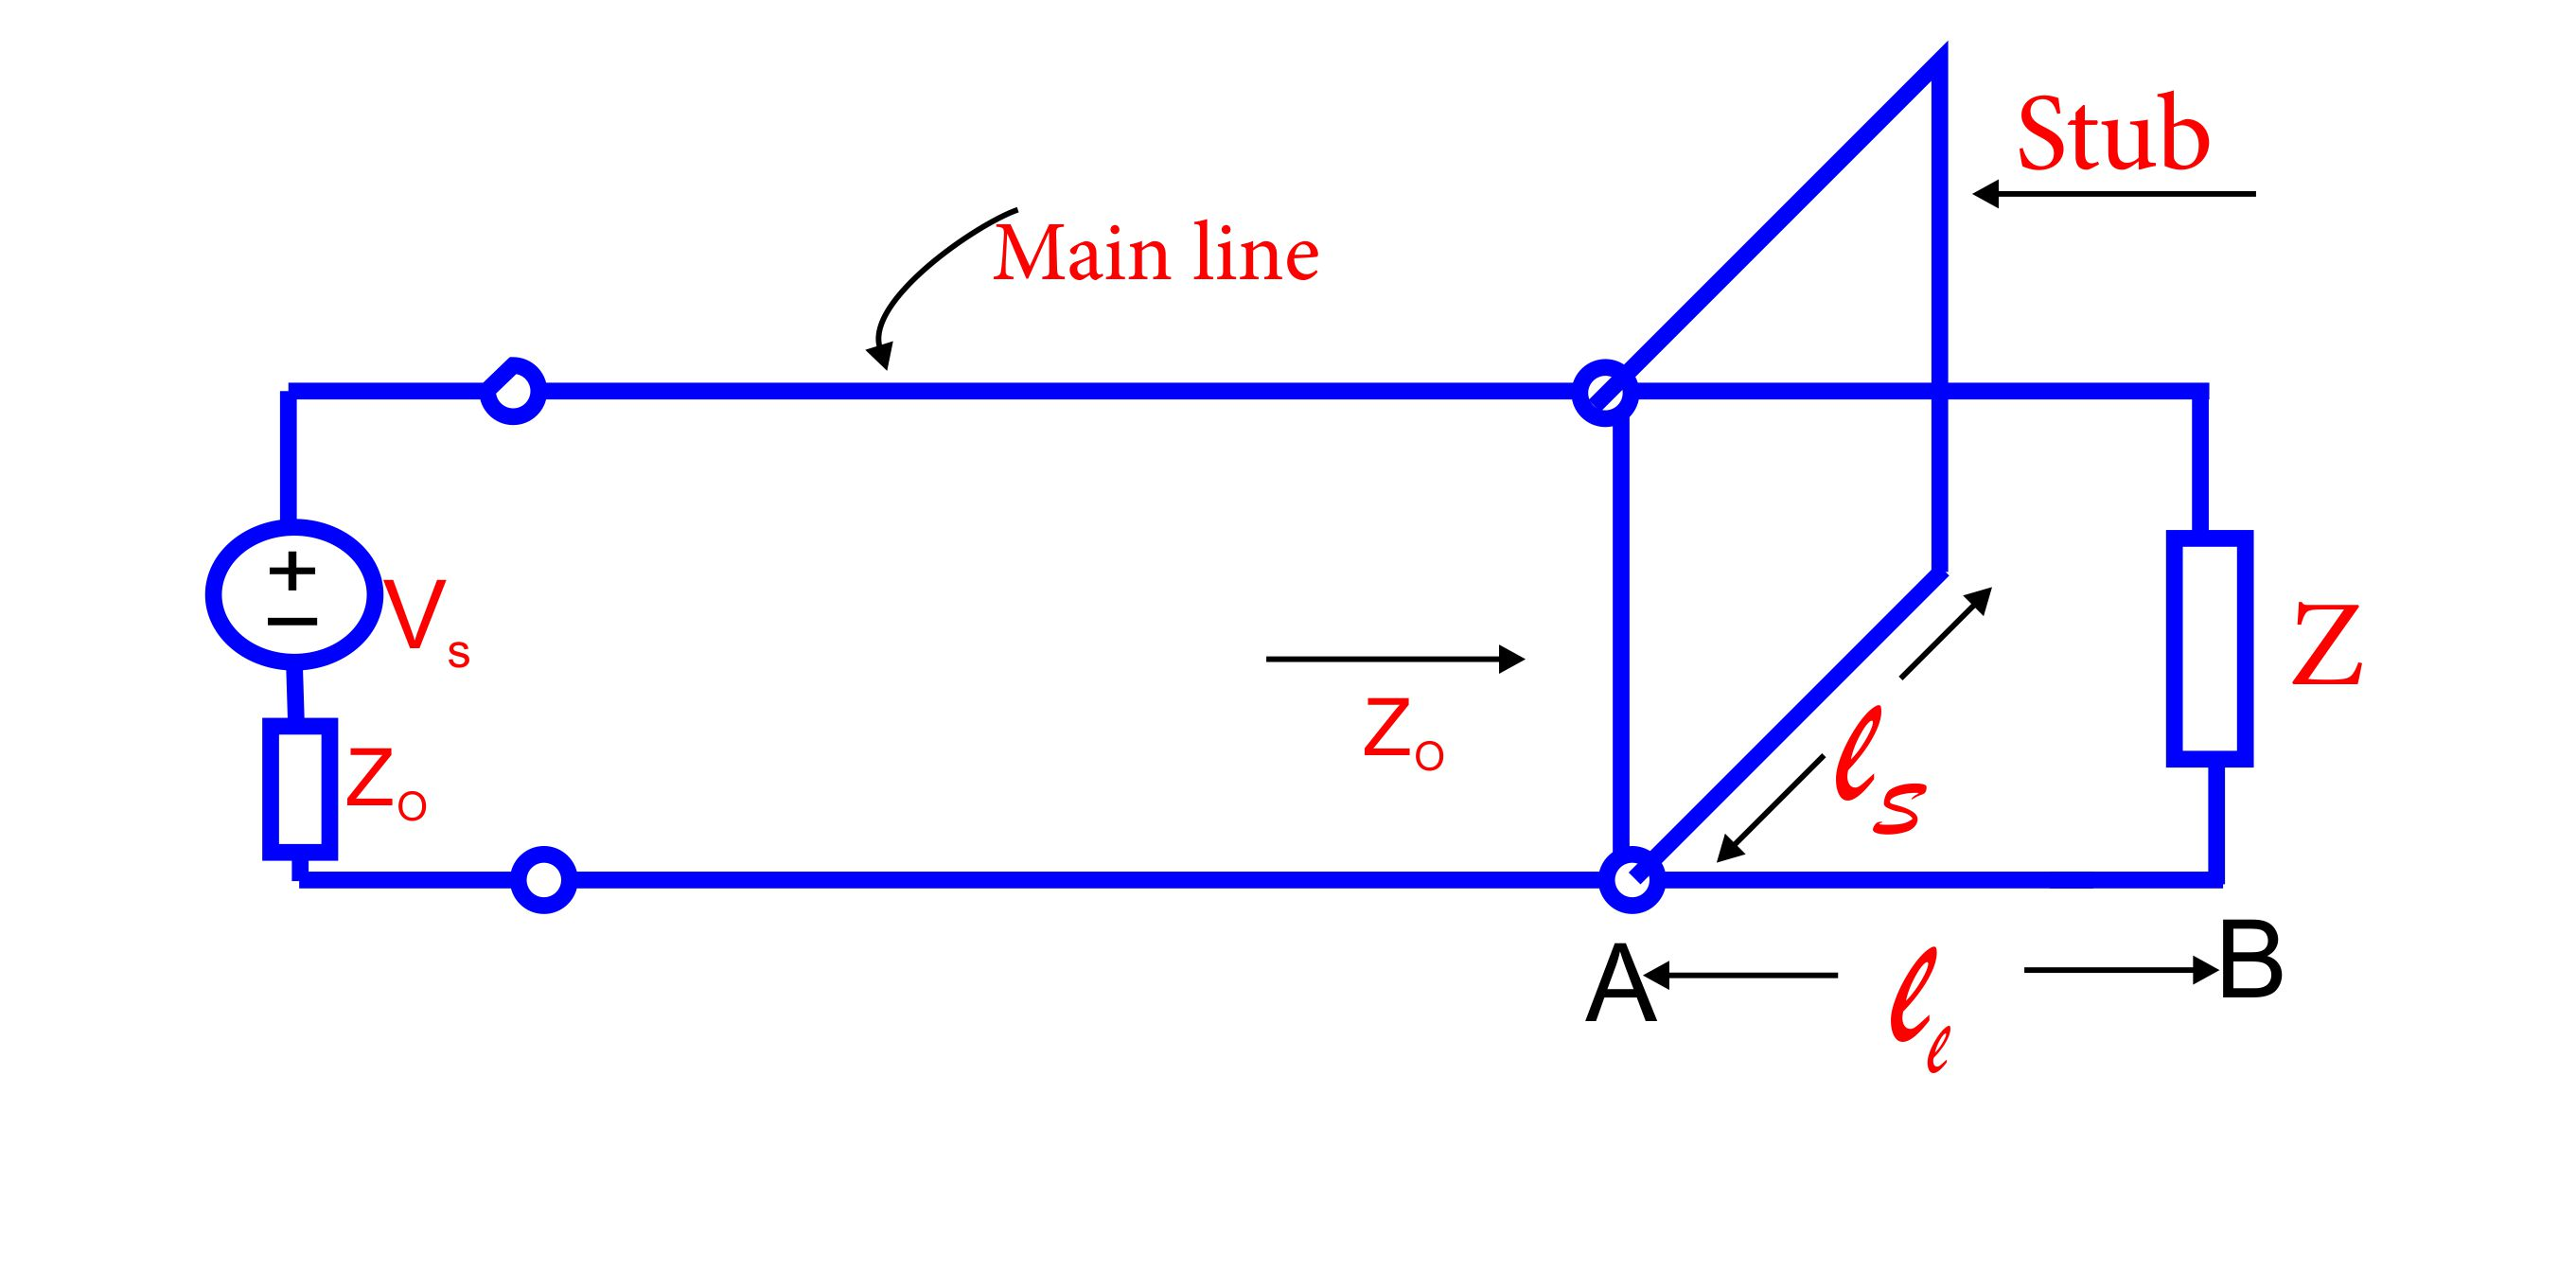
\includegraphics[width=1\linewidth]{./graphics/fig11}
\caption{Single stub matching technique with one auxiliary line attached}
\end{figure}

We are going to consider the single stub matching technique in the\textit{ parallel short circuit type.} Again, our aim is to find a real impedance at point A in figure 12.7 which is equal to $Z_o$. The main line with characteristics impedance $ Z_o$ is connected to impedance Z. We connect the auxiliary transmission line to the main transmission line. The stub is short circuited. The stub length $l_s$ is connected in parallel to the main transmission line at a distance $ l_l$ from the impedance to be matched. We know that as voltage or energy moves from generator to the load, it sees two(2) parts: the stub section and load Z section. At the load, there is  reflection and since the stub is sort circuited, there is a total reflection which is in opposite direction ($\Gamma_{s.c} = -1$). If we make sure that both reflected energy from stub and  from load match each other in amplitude and are opposite in phase, there will be no reflection beyond node A. Since there is no reflection beyond A i.e the input impedance is always going to be equal to the characteristic impedance.\\

Therefore, the solution is as follows; we need to find the length $ l_l$  such that when Z is transformed by this distance, the resistive part becomes equal to $Z_o$ and the parallel combination of the transformed impedance and the reactive part from the stub cancels out.\\

Choose $l_s$, such that the reactive part of stub cancels the reactive part of the load after its transformation. The function of Length $l$(location of stub), is to make impedance Z to be equal to characteristic impedance($Z_o$) and length of stub($l_s$) functions to neutralize the reactive part. Doing this analytically  is tedious but using smith chart is easier.\\

For single stub matching, it is better to work in terms of admittances because of the parallel connection.\\
Let load 
\begin{equation}
Y = 1/Z
\end{equation}
characteristic admittance 
\begin{equation} Y_o = 1/Z_o\end{equation} 
and normalized load admittance with respect to characteristic admittance 
\begin{equation} 
\overline{Y}=\frac{Y}{Y_o} 
\end{equation}
\textbf{Lets see how this work on the smith chart}. % put smith chart here%.
\begin{figure}[h]
\centering
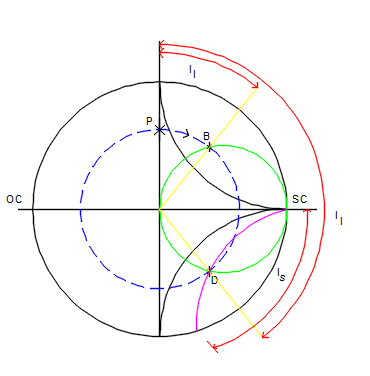
\includegraphics[width=1\linewidth]{./graphics/qwtch}
\caption{Simplified smith chart for single stub matching}
\end{figure}
Let P be the normalized admittance to be matched in figure 12.8. We draw the constant VSWR circle passing through P. When this circle intersect g = 1 circle, at that point it means the real part will be equal to the characteristic impedance $Z_o$. i.e. at point (B and D). Distance (P to B) or (P to D) will give us what the reactive
part should be at that location since we know already the conductive part is equal to 1. The distance PB = $l_l$ from figure 12.7 or the distance PD will serve the same purpose. At A, \footnote{$Y = g + jb$}$\overline{Y} = 1 + jb' $. Then the stub must have $-jb'$ as its admittance so that when they are connected in parallel, the susceptance cancels out leaving only the normalize admittance of $1 + j0$.
Also when the stub is connected in series, we use the same pattern but we will use impedance values instead of admittances.\\
The process involved are:\\
\begin{itemize}
\item[a.]First locate the given admittance value to be matched on the smith chart.
\item[b.]Draw your constant VSWR circle  around the located point on smith chart.
\item[c.] Move on the constant VSWR circle in a clockwise direction and mark the two points it intersect with the constant g = 1 circle.
\item[d.]The distance from the first location (point P) to either of these new points (point B or D) is the location of stub $l_l$.
\item[f.] Choosing point B (1+j$b'$), take a mirror image which is point D(1 - j$b'$). Draw a constant susceptance circle passing through this point D. Where this circle touches the outermost circle of smith chart is$ -jb'$.
\item[g.] The distance moving anticlockwise\footnote{Since stub is S.C, energy is totally reflected.} from this point S to the S.C point on the smith chart give us the length of stub.
\end{itemize}

Single stub matching technique is an extremely useful technique in matching impedances to the characteristics impedance of the line. In this technique, we are matching impedance without any unique \textbf{Transmission line} as in the case of a Quarter wavelength transformer technique.\\

However, this technique has a small drawback which is: the location of the stub  depends on the impedance to be matched. Though the single stub technique can match all possible load, for every load to be matched, the location of the stub has to be changed which may not be that easy once the stub is connected.\\

To solve this limitations as we did for quarter wavelength transformer technology, we will use the Double stub matching technique.
\subsection{Double Stub Matching Technique}

This technique involves the use of two(2) stub. In this method, we change only the length of the stub while the location of stub is fixed. The separation between the stubs is $ 3\lambda/8$. The distance between stub 1 and load is $l_l$%put footnote here and two figures(double stub(12.9) and smith chart(12.10))%
\begin{figure}[h]
\centering
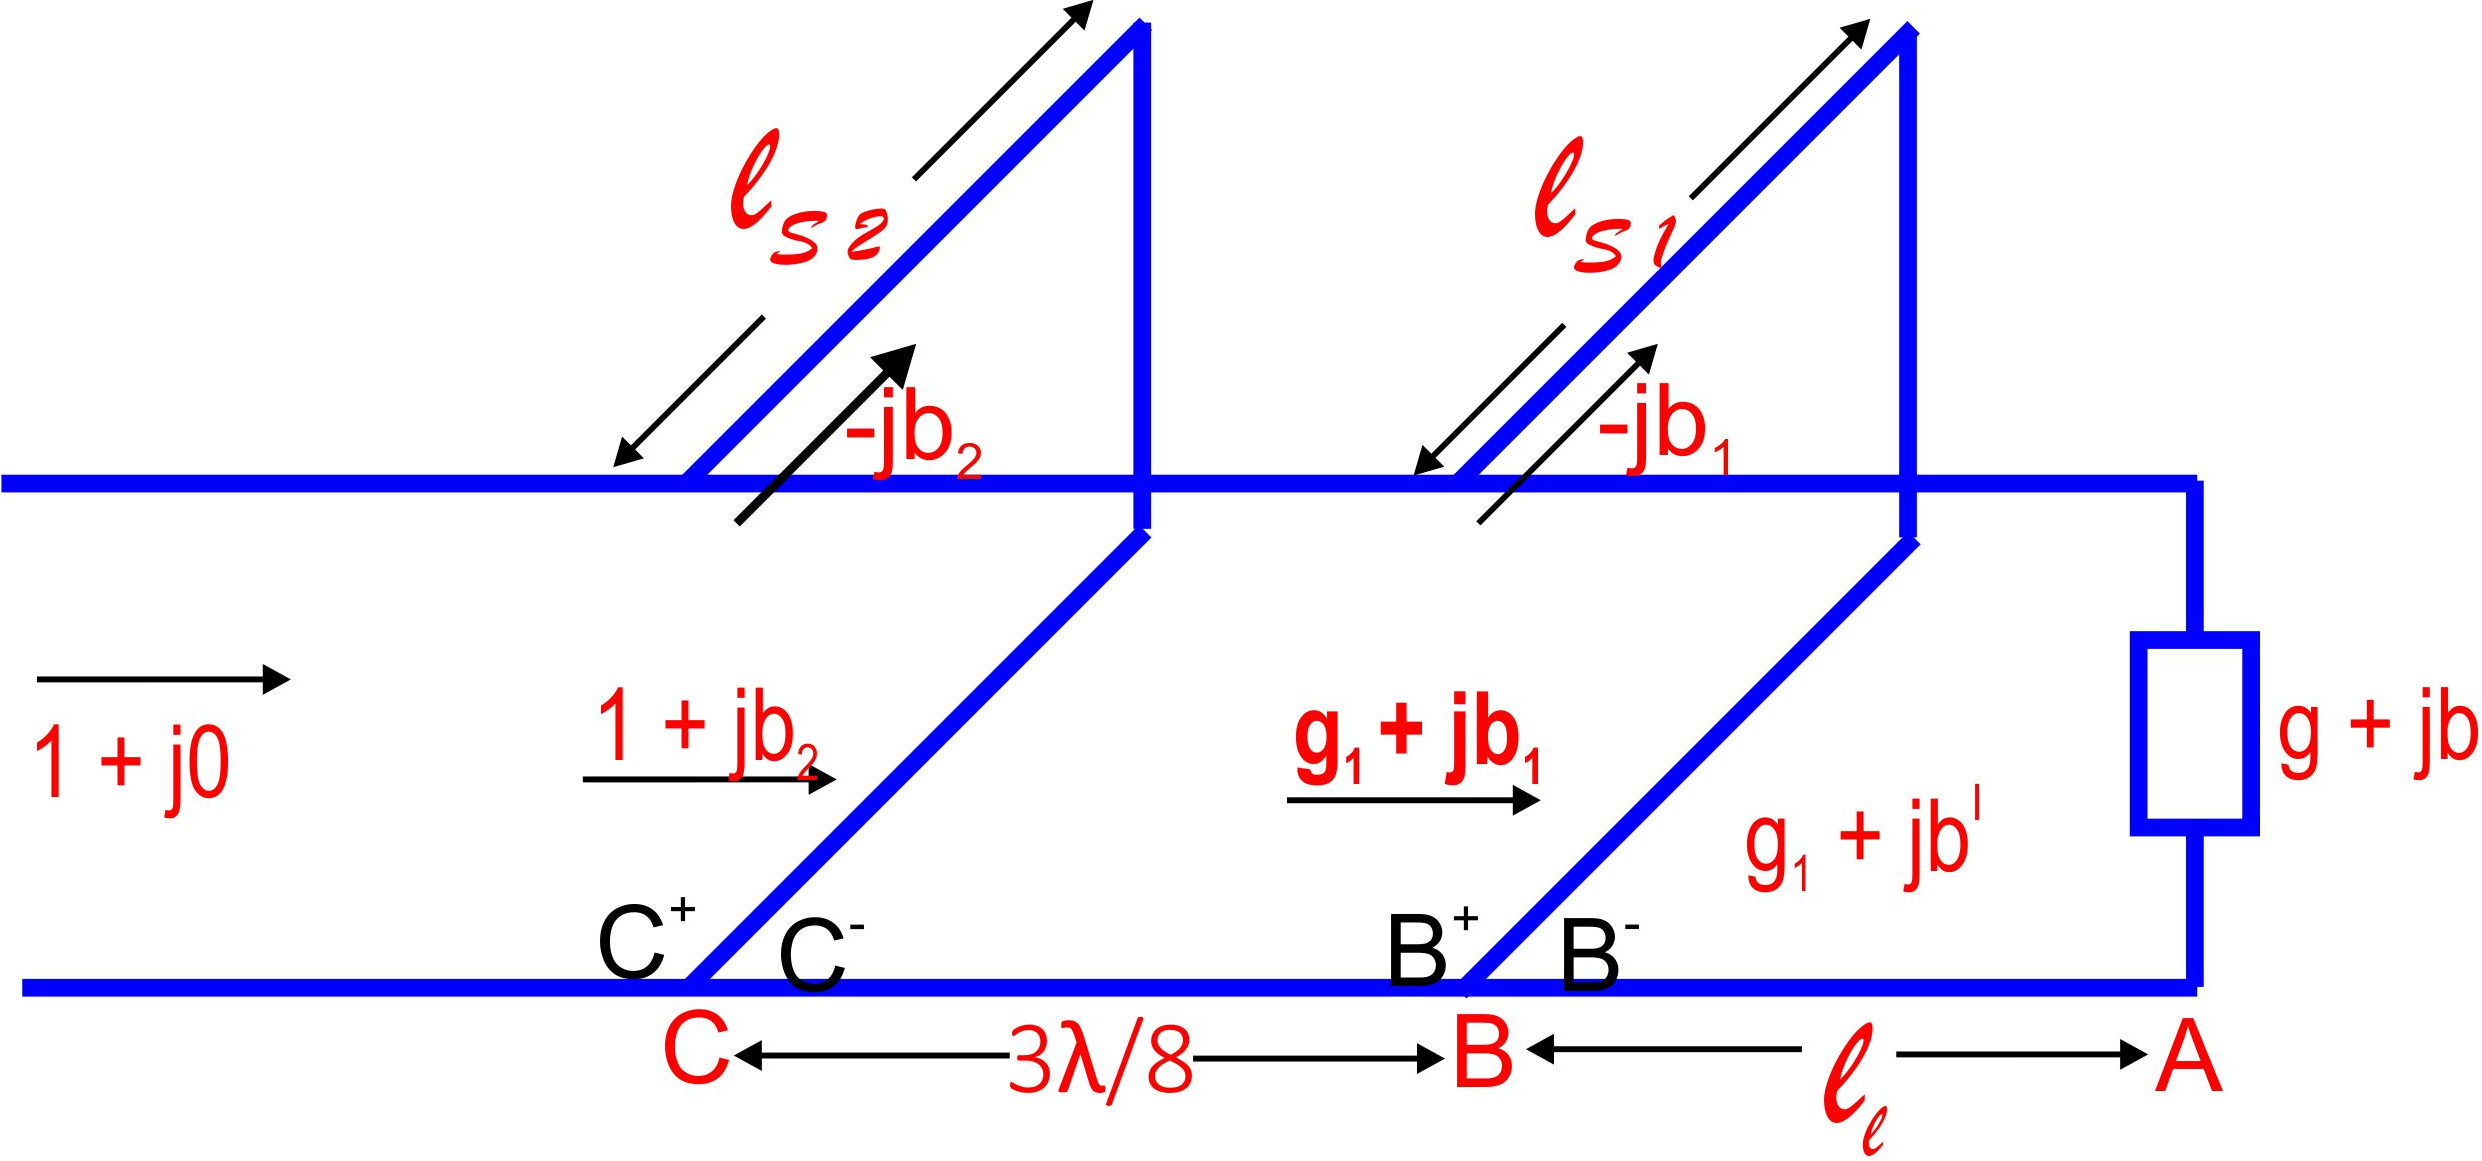
\includegraphics[width=1\linewidth]{./graphics/fig12}
\caption{Double stub matching technique with two auxiliary lines attached}
\end{figure}
\begin{figure}[h]
\centering
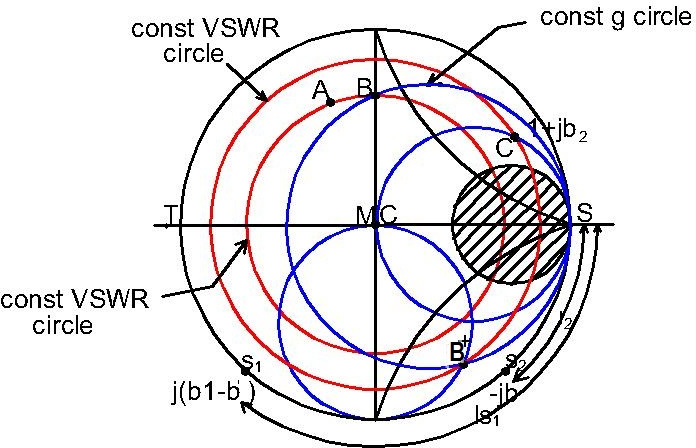
\includegraphics[width=1\linewidth]{./graphics/dousmith}
\caption{Simplified smith chart for double matching technique}
\end{figure}\\
\underline{\textbf{Procedure:} } \\

From figure 12.9, starting from the output, the initial Admittance was $g + jb$. After a distance $l_l$ moving clockwise to point B (towards generator ), (at this point $B = g' + jb'$) when this is combined with the susceptance from the stub($-jb_1$), we get $g_1 +jb_1$. When transformed along the length $3\lambda/8$, we get 1 + $jb_2$. When this is combined with the susceptance of stub 2$(-jb_2)$, we get $1 + 0j$ beyond point $C^+$.\\

Using smith chart for the analysis, since we are to move a distance of $3\lambda/8$, we first rotate circle g = 1  by $270^o$. Mark the normalized admittance $g + jb$  (since we are dealing with parallel circuit) denoted by A on figure 12.10. Move by $l_l$ to get to point B(g + j$b'$). At point B, since we are adding a stub of $-jb'$, we are changing only the reactive part. So we move anticlockwise on the constant conductance circle till we get to the rotated g = 1 circle. At this point, we now move on a constant VSWR circle in a clockwise direction, i.e. we move by $ 3\lambda/8$. After the distance $ 3\lambda/8$, the point touches the initial g = 1 circle given by point $C (1+ jb_2$). To cancel $jb_2$ you take a mirror image of $1-jb_2$, then find conductance circle of $ -jb_2$ at the outermost circle of the smith chart. We measure the distance from this point to the S.C point in an anticlockwise direction to give us the length of the second stub.\\

Now to find the length of the first stub, we find the difference between the two (2) susceptance value $B$ and $B^+$, since the conductance are the same. Mark the difference on the outermost circle of smith chart($S_1$). The distance from this point to the S.C point moving anticlockwise gives the length of the first stub. \\

However, this has a small drawback which is, the whole essence of matching is possible provided that by moving in a constant conductance circle we can intersect the $g = 1$ circle. If by the movement through the constant conductance circle we can not reach the rotated $g = 1$ circle, then the matching is not possible. Now we know the nature of the constant g circle (that they are within another). So it is possible that if the admittance at point B lies in a circle smaller than the $g = 1$ circle, then by our movement inside the constant conductance circle, we will never be able to come to the rotated g = 1 circle. If we can not come to the rotated $g = 1$ circle, then the impedance after transformation can not come to the original $g =1$ circle i.e. matching is not possible. What this means is that if $g' + jb'$ lies within the shaded forbidden region shown in figure 12.10, then the impedance matching is not possible. The impedance we want to match can lie in the forbidden region, but the transformed impedance after distance $ l_l$ should be out of the forbidden region.\\

So by choosing a proper value for $l_l$, we can avoid the forbidden region. Therefore, the double stub matching technique has a small limitation that it cannot match those impedances whose transformed value after $l_l$ lie within the forbidden region. However, this has been solved by introducing the concept of three stub matching.
\begin{figure}[h]
\centering
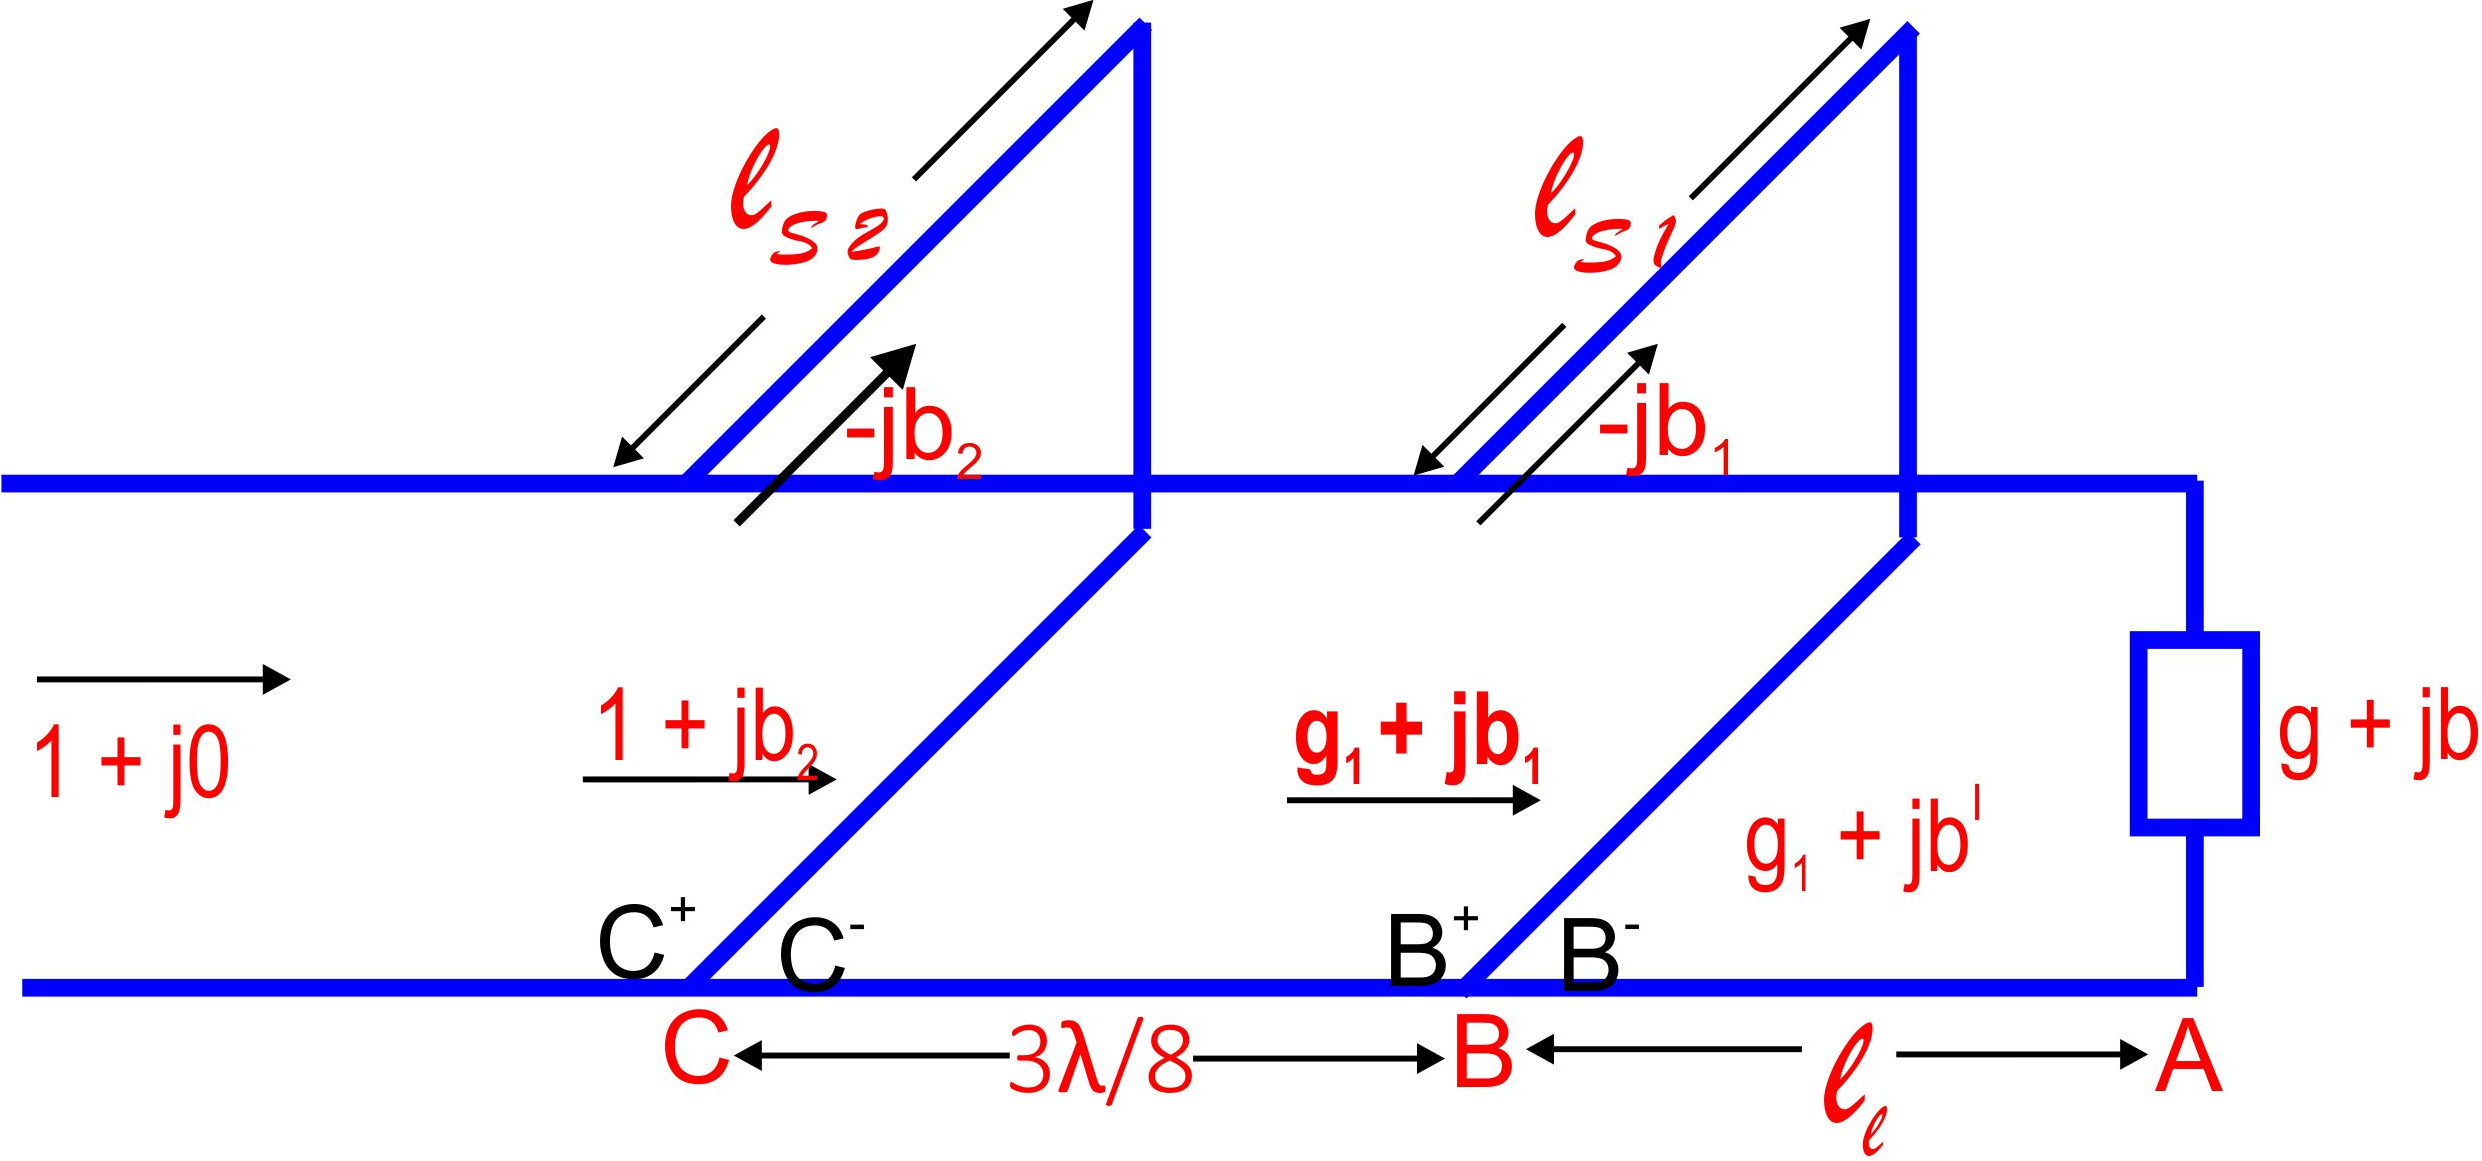
\includegraphics[width=1\linewidth]{./graphics/fig12}
\caption{Double stub matching technique with two auxiliary lines attached}
\end{figure} 

\begin{exmp}
For a load $Z_{o} = 50ohms$, $Z_{L} = (100 + j100)ohms$ design a double stub machine to match the load for the transmission line.Note $l_{1} = 0.4\lambda$
\subsection{Solution}
$$\bar{Z_{L}} = \frac{Z_{L}}{Z_{o}} = 2 + j2$$
Note:$\frac{3\lambda}{8}$ correspond to $270^{o} $ rotation on the smith chart.Because 0.5$\lambda$ correspond to $ 360^{o}$. 
\begin{figure}[h]
\centering
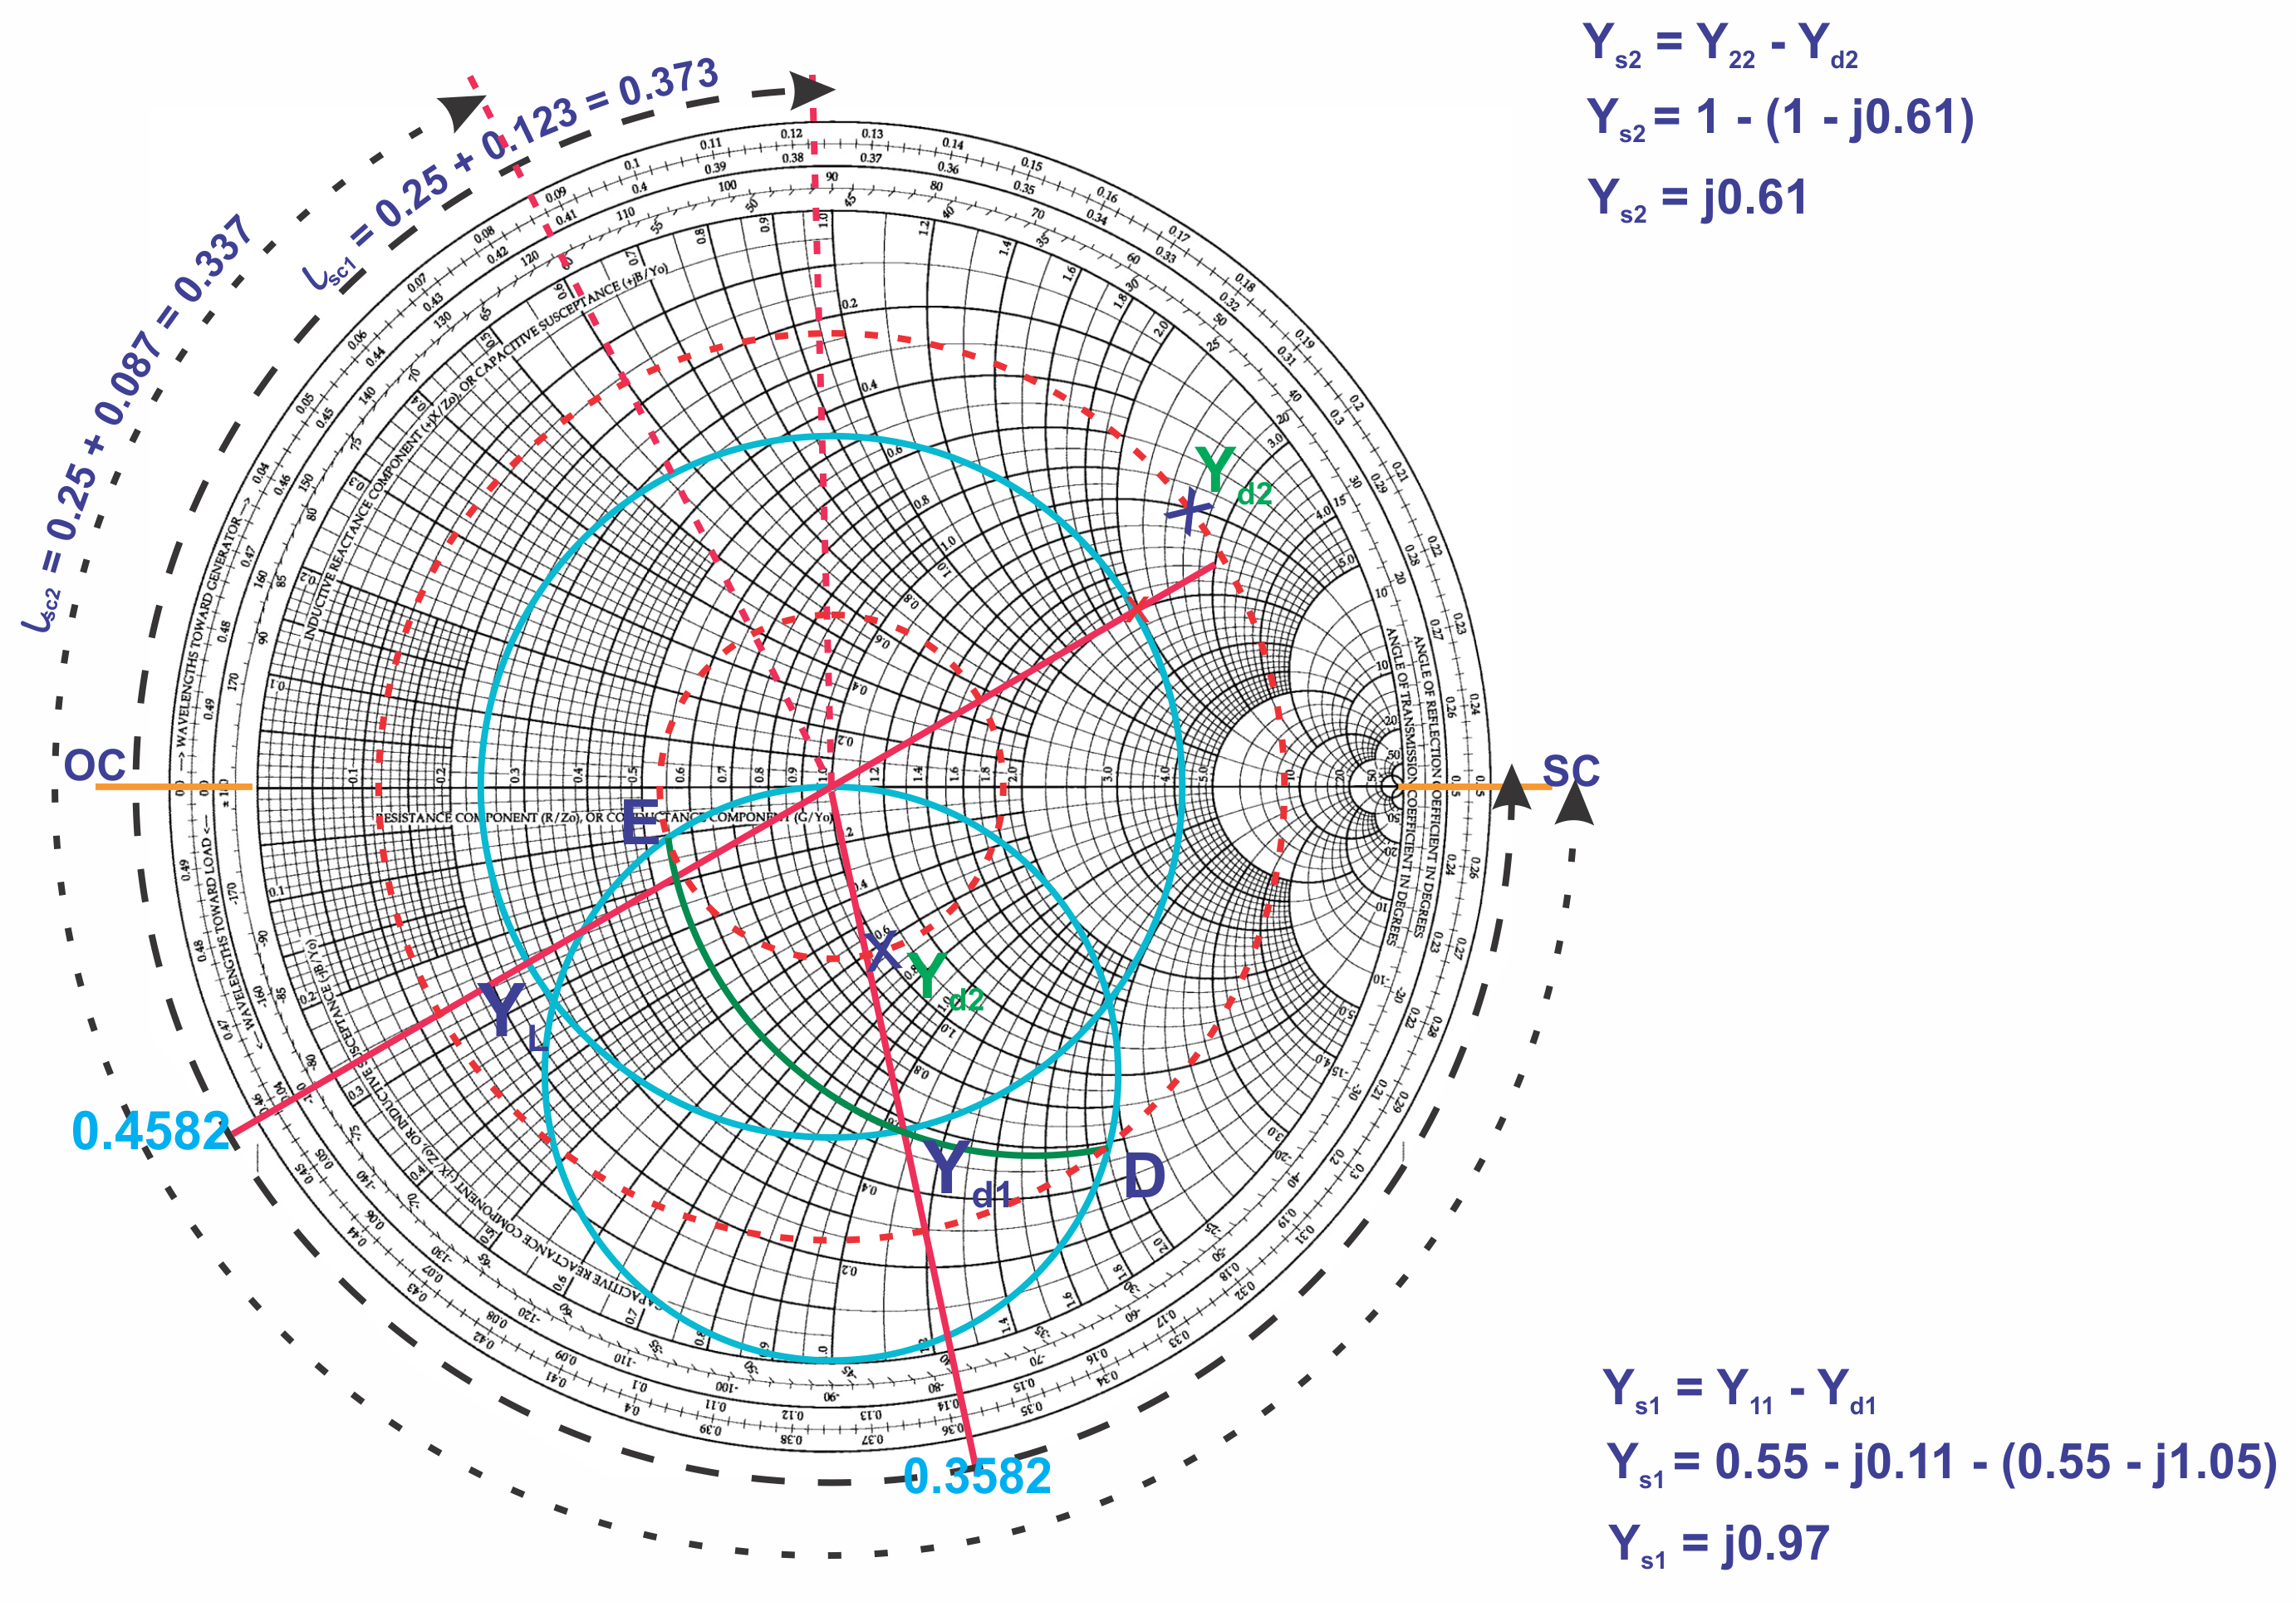
\includegraphics[width=1\linewidth]{./graphics/question1}
\caption{worked example}
\end{figure}
				
\textbf{PROCEDURES:}
\begin{enumerate}
\item Determine the normalized value for the load resistance $Z_{L}$. Using $\overline{Z_{L}} = \frac{Z_{L}}{Z_{o}}$ 
\item Mark the point on the smith chart $\overline{Z_{L}} = 2 + j2$   
\item Draw the constant VSWR circle from the normalized impedance point
\item Move $180^{o}$ from the normalized impedance point on the constant VSWR circle to the normalized admittance $Y_{L}$
\item Extend the point $Y_{L}$ to meet the bigger circle on the smith chart 
\item Where the line meets the VSWR circle mark the point and name it $Y_{d1}$                       
\item Draw a rotated $270\deg $ circle of radius 1                                                  
\item At point $Y_{d1}$, moving at constant g mark point E and D which cuts the rotated $270\deg $ circle of radius 1 at point ends.
\item Point E and D are $Y_{11}$                                                
\item Solve for $Y_{s1}$ (Using either point E and D as $Y_{11}$) $Y_{s1}$ =    $Y_{11}$ -    $Y_{d1}$                     
\item Mark point $Y_{s1}$ on the smith chart, extend the point to the circle and measure its wave length  towards the generator $l^{1}$ 
\item Moving from short circuit point to point $Y_{s1}$. Calculate the distance
$ l_{s1} = 0.25 + l^{1} $                                                                        
\item To get $l_{s2}$. With radius from center to point E, draw a circle and with radius from center to point D draw a circle
\item Mark the $270\deg$ point of radius point E circle, where it meets with the unit resistance circle, mark the point and call it $Y_{d2}$. With radius from center to point D mark the $270\deg$ point, where it meets with the unit resistance circle and call it $Y_{d2}^{1}$ 
\item With point $Y_{d2}$ or $Y_{d2}^{1}$ get $Y_{s2}$ $Y_{22}=1$ $Y_{s2}=Y_{22}-Y_{d2}^{1}$
\item Mark the point $Y_{d2}$ on the smith chart and extend to the outer circle. Mark the point $l^{11}$
\item Measure the length from the short circuit point to the $l^{11}$ $Y_{d2} = 0.25 + l^{11}$
\end{enumerate}
\end{exmp}

\begin{figure}[h]
\centering
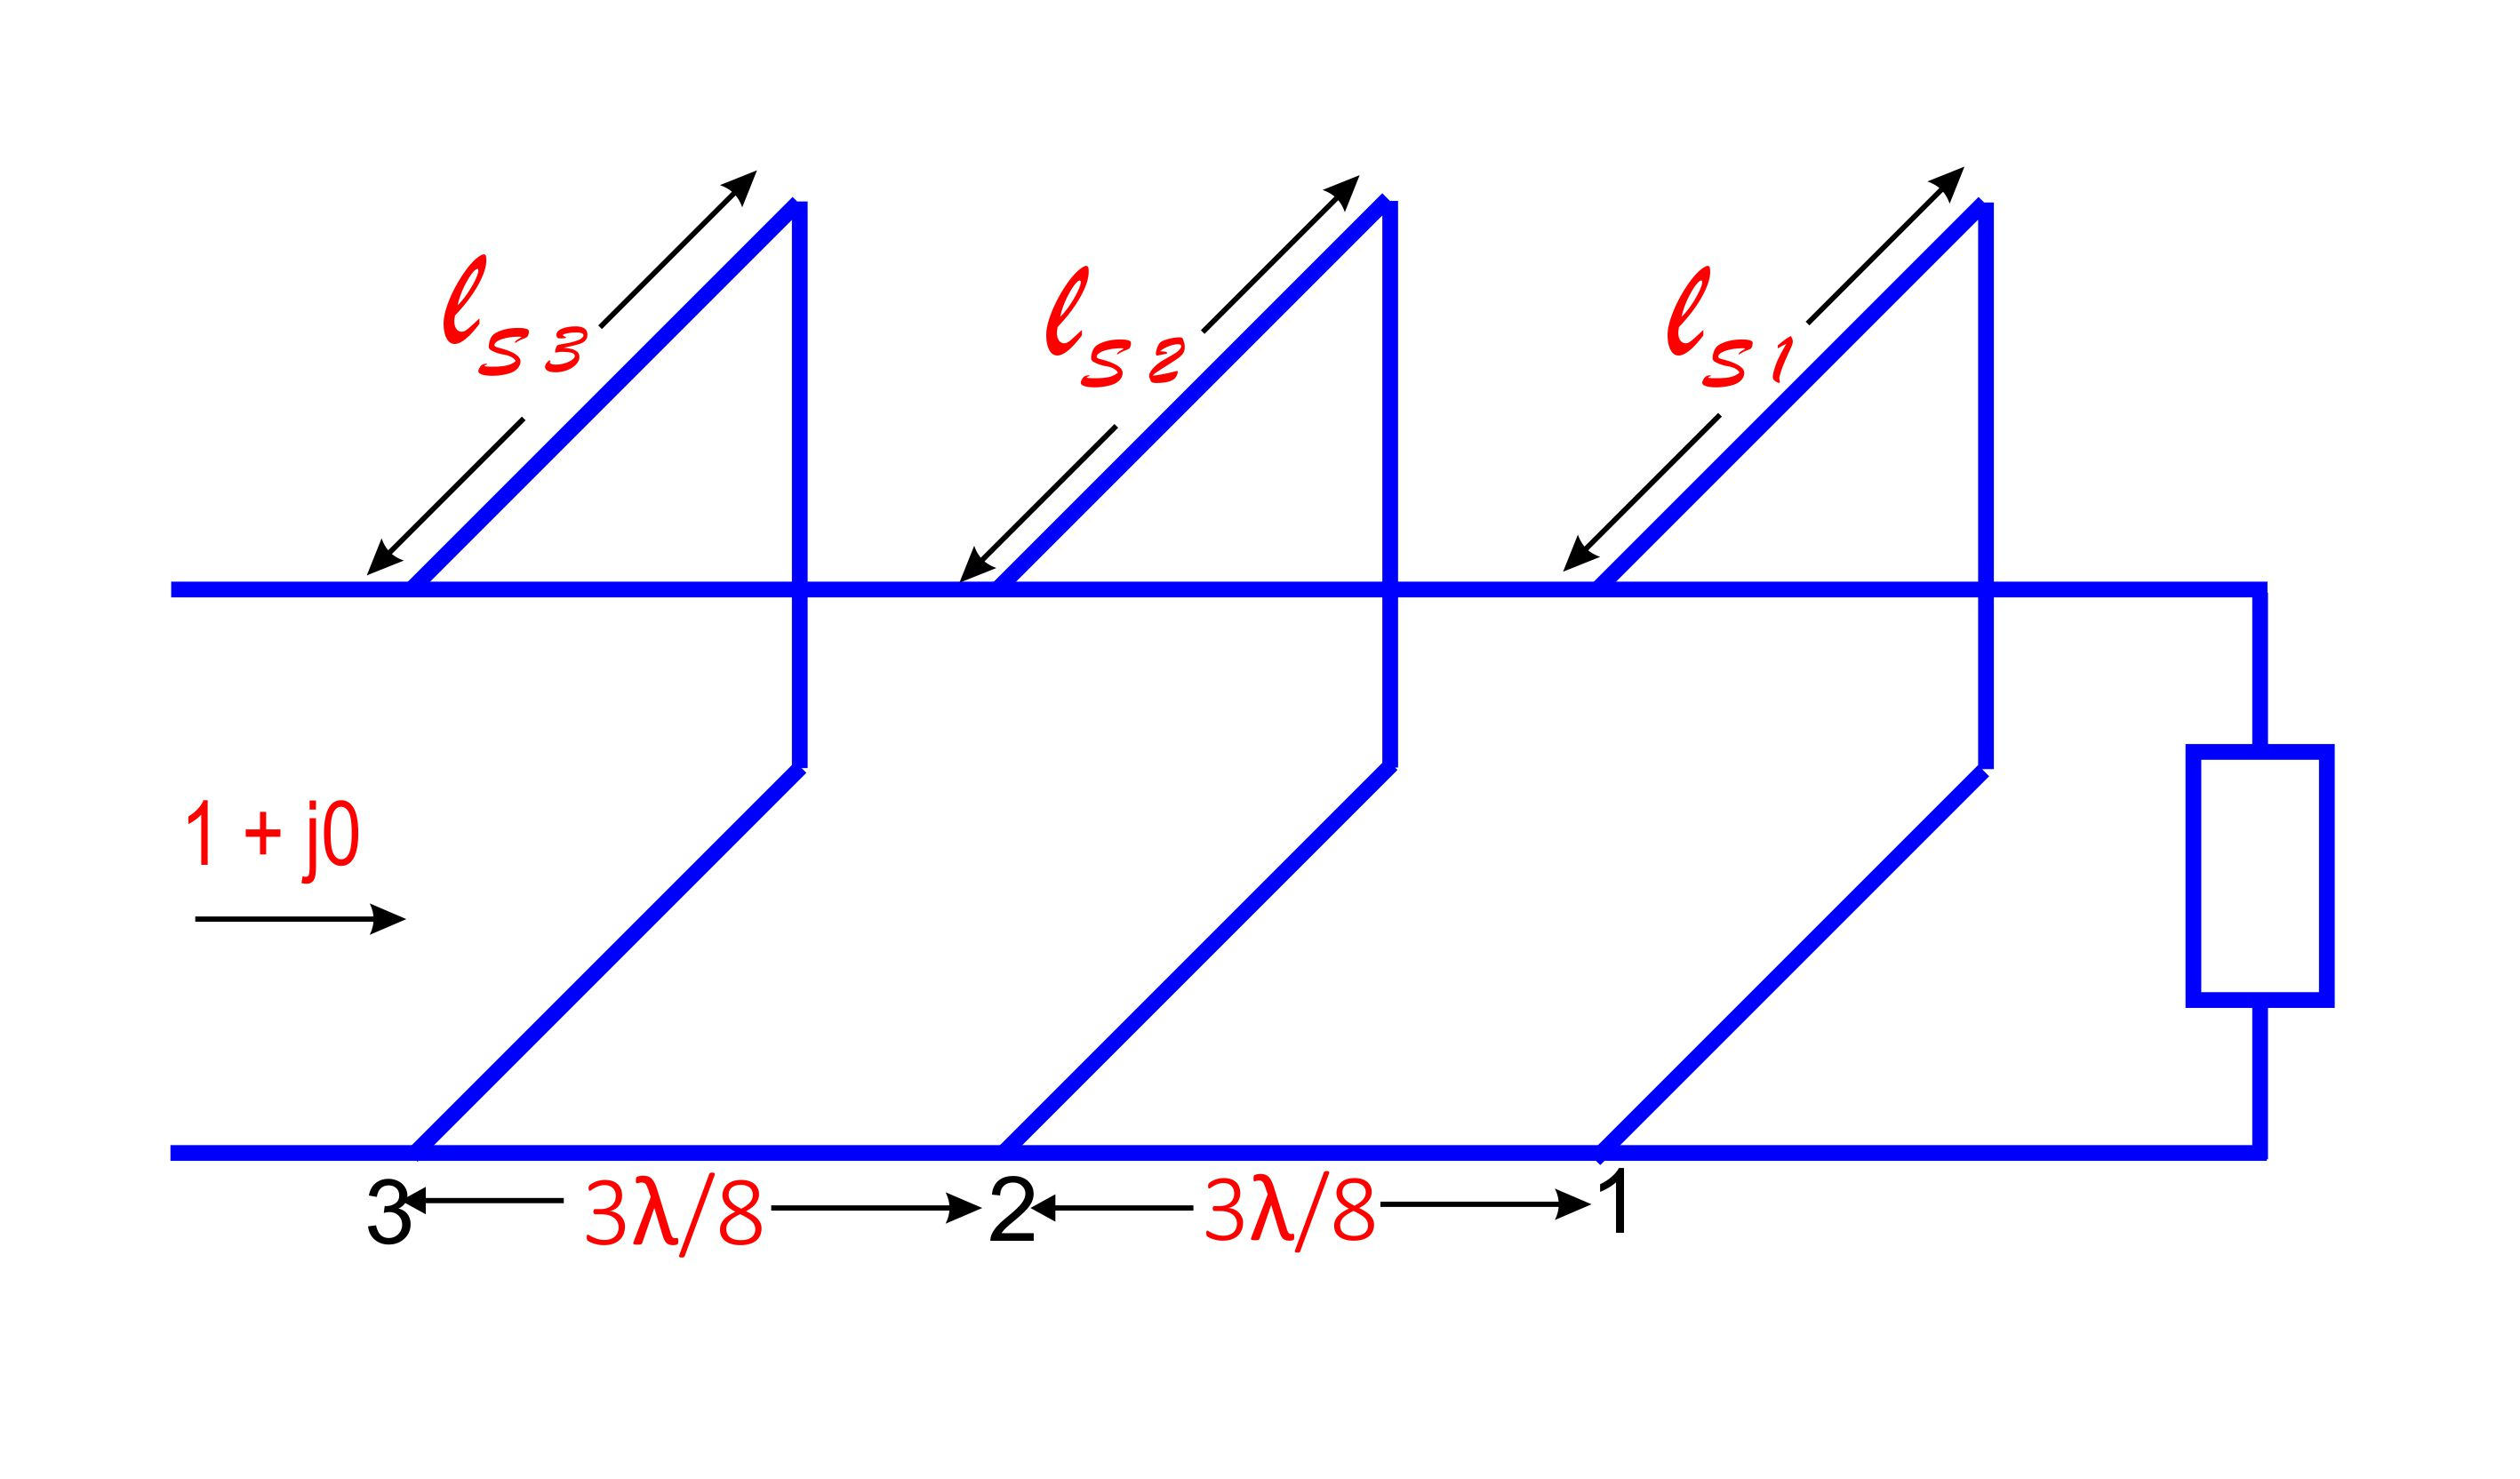
\includegraphics[width=1\linewidth]{./graphics/fig13}
\caption{Three stub matching technique with three auxiliary lines attached}
\end{figure}

From figure 12.11, if the matching is done with stub 2 and 1 and stub 3 is made an open circuit (so that the $ l_{s3}$ equals quarter wavelength), we find that stub 2 and 3 makes the transformed impedance to lie in the forbidden region.So we disconnect stub 3 and make use of stub 1 and 2. Depending on whether the transformed impedance lie within the forbidden region or not, we can make use of stub 1 and 2 or stub 2 and 3. 

The final solution in the impedance matching is the three stub technique. By using this method, all possible impedances can be matched without moving the location of the stub on the transmission line.

In conclusion,  we have dealt with the major application of \textit{transmission line} which is, impedance matching in which we covered the different methods with which impedance can be matched. These are:
\begin{enumerate}
\item The quarter wavelength matching technique.
\item Single stub matching technique.
\item Double stub matching technique and
\item The triple stub matching technique.
\end{enumerate}

At the end we resolved that the triple stub matching technique is the best technique among all the techniques.
